%============================================================================
% tento soubor pouzijte jako zaklad
% (c) 2008 Michal Bidlo
% E-mail: bidlom AT fit vutbr cz
%============================================================================
% kodovaní: UTF-8 (zmena prikazem iconv, recode nebo cstocs)
%----------------------------------------------------------------------------
% zpracování: make, make pdf, make clean
%============================================================================
% Šablonu upravil: Ing. Jaroslav Dytrych, idytrych@fit.vutbr.cz
%============================================================================
\documentclass[]{fitthesis} % bez zadání - pro začátek práce, aby nebyl problém s překladem
%\documentclass[zadani]{fitthesis} % odevzdani do wisu - odkazy jsou barevné
%\documentclass[zadani,print]{fitthesis} % pro tisk - odkazy jsou černé
%\documentclass[english,print]{fitthesis} % pro tisk - odkazy jsou černé
% * Je-li prace psana v anglickem jazyce, je zapotrebi u tridy pouzit 
%   parametr english nasledovne:
%      \documentclass[english]{fitthesis}
% * Je-li prace psana ve slovenskem jazyce, je zapotrebi u tridy pouzit 
%   parametr slovak nasledovne:
%      \documentclass[slovak]{fitthesis}

\usepackage[czech,slovak,english]{babel}
\usepackage[utf8]{inputenc} %kodovani
\usepackage[T1]{fontenc}
\usepackage{cmap}
\usepackage{url}
\DeclareUrlCommand\url{\def\UrlLeft{<}\def\UrlRight{>} \urlstyle{tt}}

%zde muzeme vlozit vlastni balicky
\usepackage{listings}
\usepackage[toc,page,header]{appendix}
\RequirePackage{titletoc}
\ifczech
  \usepackage{ae}
\fi
\usepackage{amsmath}
\usepackage{xr}
\usepackage{tikz}
\usepackage{subcaption}
\usepackage{pgfplots}
\usetikzlibrary{pgfplots.statistics}
\usepackage{algpseudocode}
\usepackage{algorithmicx}
\usepackage{algorithm}
\usepackage{amssymb}
\usepackage[final]{pdfpages}



\input{pisma.tex}

% vypne funkci nové šablony, která automaticky nahrazuje uvozovky,
% aby nebyly prováděny nevhodné náhrady v popisech API apod.
\csdoublequotesoff

% =======================================================================
% balíček "hyperref" vytváří klikací odkazy v pdf, pokud tedy použijeme pdflatex
% problém je, že balíček hyperref musí být uveden jako poslední, takže nemůže
% být v šabloně
\ifWis
\ifx\pdfoutput\undefined % nejedeme pod pdflatexem
\else
  \usepackage{color}
  \usepackage[unicode,colorlinks,hyperindex,plainpages=false,pdftex]{hyperref}
  \definecolor{links}{rgb}{0.4,0.5,0}
  \definecolor{anchors}{rgb}{1,0,0}
  \def\AnchorColor{anchors}
  \def\LinkColor{links}
  \def\pdfBorderAttrs{/Border [0 0 0] }  % bez okrajů kolem odkazů
  \pdfcompresslevel=9
\fi
\else % pro tisk budou odkazy, na které se dá klikat, černé
\ifx\pdfoutput\undefined % nejedeme pod pdflatexem
\else
  \usepackage{color}
  \usepackage[unicode,colorlinks,hyperindex,plainpages=false,pdftex,urlcolor=black,linkcolor=black,citecolor=black]{hyperref}
  \definecolor{links}{rgb}{0,0,0}
  \definecolor{anchors}{rgb}{0,0,0}
  \def\AnchorColor{anchors}
  \def\LinkColor{links}
  \def\pdfBorderAttrs{/Border [0 0 0] } % bez okrajů kolem odkazů
  \pdfcompresslevel=9
\fi
\fi

%Informace o praci/projektu
%---------------------------------------------------------------------------
\projectinfo{
  %Prace
  project=DP,            %typ prace BP/SP/DP/DR
  year=2016,             %rok
  date=\today,           %datum odevzdani
  %Nazev prace
  title.cs={Evoluční návrh hašovacích funkcí},  %nazev prace v cestine
  title.en={Evolution design of hash functions}, %nazev prace v anglictine
  %Autor
  author={Marek Kidoň},   %jmeno prijmeni autora
  author.title.p=Bc., %titul pred jmenem (nepovinne)
  author.name={Marek},   %jmeno autora (pro citaci)
  author.surname={Kidoň},   %prijmeni autora (pro citaci)
  %Ustav
  department=UPSY, % doplnte prislusnou zkratku dle ustavu na zadani: UPSY/UIFS/UITS/UPGM
  %Skolitel
  supervisor= Roland Dobai, %jmeno prijmeni skolitele
  supervisor.title.p=Ing.,   %titul pred jmenem (nepovinne)
  supervisor.title.a={Ph.D.},    %titul za jmenem (nepovinne)
  supervisor.name={Roland},   %jmeno skolitele (pro citaci)
  supervisor.surname={Dobai},   %prijmeni skolitele (pro citaci)
  %Klicova slova, abstrakty, prohlaseni a podekovani je mozne definovat 
  %bud pomoci nasledujicich parametru nebo pomoci vyhrazenych maker (viz dale)
  %===========================================================================
  %Klicova slova
  keywords.cs={	evoluční návrh
  	, hašovací funkce
  	, genetické programování
  	, počítání podle přírody
  	, internetový protokol
  }, %klicova slova v ceskem jazyce
  keywords.en={ evolution design
  	, hash function
  	, genetic programming
  	, natural computing
  	, internet protocol
  }, %klicova slova v anglickem jazyce
  %Abstract
  abstract.cs={
  	Hašovací tabulky jsou rychlé vyhledávací struktury, které se staly součástí
  	moderního světa výpočetních technologií a svou snadnou implementací si získali
  	mnoho příznivců v řadách programátorů. Volba vhodné hašovací funkce je klíčová.
  	Nevhodně zvolená hašovací funkce může mít za následek špatný výkon hašovací tabulky
  	a aplikace na ní navázanou. 
  	% continue
  	V současné době existují velmi dobré implementace obecných hašovacích funkcí, tedy
  	takových, jejichž vstup není omezen na konkrétní doménu. Na druhé straně, pokud
  	známe vstupní doménu, můžeme navrhnout hašovací funkcí na míru dané aplikaci a tím
  	dosáhnout výrazně lepších výsledků než v případě hašovací funkce obecné.
  	% problem
  	Návrh hašovací funkce není triviální záležitost. Neexistují pevně dané normy,
  	pravidla, návody ani automatizované nástroje, který by za nás tuto práci odvedly.
  	V případě ručního návrhu se autor hašovací funkce musí spoléhat na své znalosti,
  	zkušenosti, vynalézavost a intuici. 
  	% approach
  	V případě takto komplikovaných úloh je někdy vhodné se uchýlit k méně tradičním 
  	technikám návrhu jako jsou evoluční algoritmy. Evoluční algoritmy přistupují	 
  	k řešení problémů způsobem prohledávání stavového prostoru,
  	který se inspiruje v přírodních procesech, a to konkrétně v Darwinistické reprodukci druhů. 
  	% solution design
  	V této práci se budeme zabývat evolučním návrhem hašovacích funkcí pro doménu
  	\textit{IP} adres, unikátních identifikátorů síťového rozhraní v sítích řízených
  	internetovým protokolem. Vybraným evolučním algoritmem je genetické programování, velmi
  	specifická podskupina počítání podle přírody, která svými vlastnosmi umožňuje 
  	navrhnovat skutečně kvalitní hašovací funkce.
  	% results
  	Evolučně navržené hašovací funkce nabízejí velmi dobré vlastnosti s ohledem na 
  	specifickou aplikaci. A předčí své \textit{state-of-the-art} obecné, člověkem navržené
  	protějšky co se rychlosti i odolnosti vůči kolizím týče.
  }, % abstrakt v ceskem jazyce
  abstract.en={ % motivation
  	Hash tables are fast associative array implementations which became part of modern
  	world of information technology and thanks to its simplicity became very popular 
  	among computer programmers. The choice of proper hash function is very important.
  	Improperly selected hash function can result in poor hash table performance and its
  	application.
  	% continue
  	Currently there are many exceptional implementations of general hash functions. Such
  	functions are not constrained to a concrete set of inputs, they perform on any
  	input. On the other hand if we know the input domain we can design a specific hash 
  	function for desired application thus reaching better levels of performance compare to
  	a general hash function. 
  	% problem
  	However hash function design is not trivial. There are no rules, standards, guides nor
  	automated tools that would help us with such a task. In case of manual design the hash
  	function author has to rely on his/her knowledge, experience, inventiveness and 
  	intuition.  
  	% approach
  	In case of such complicated tasks there is sometimes advantageous to choose a different
  	path and use techniques such as evolution algorithms. Natural computing is an approach
  	of certain problem solutions that are inspired by the process of species reproduction as
  	defined by Charles Darwin.
  	% solution design
  	In this thesis we will design hash functions for the domain of \textit{IP} addresses,
  	that serve as an unique network device interface identifier in internet protocol networks.
  	The chosen subset of 
  	natural computing is the genetic programming, a very specific technique that is an adequate 
  	approach to our problem thanks to its properties. 
  	% results
  	Evolutionary designed hash functions offer good properties. They outperform state-of-the-art
  	generic, human-created hash functions in terms of speed and collision resistance.\newpage				 
  }, % abstrakt v anglickem jazyce
  %abstract.cs={Výtah (abstrakt) práce v českém jazyce.}, % abstrakt v ceskem ci slovenskem jazyce
  %abstract.en={Výtah (abstrakt) práce v anglickém jazyce.}, % abstrakt v anglickem jazyce
  %Prohlaseni
  declaration={Prohlašuji, že jsem tuto diplomovou práci vypracoval samostatně pod vedením pana Rolanda Dobaie},
  %Podekovani (nepovinne)
  %acknowledgment={Zde je možné uvést poděkování vedoucímu práce a těm, kteří poskytli odbornou pomoc.} % nepovinne
}

%Abstrakt (cesky, slovensky ci anglicky)
%\abstract[cs]{Do tohoto odstavce bude zapsán výtah (abstrakt) práce v českém (slovenském) jazyce.}
%\abstract[en]{Do tohoto odstavce bude zapsán výtah (abstrakt) práce v anglickém jazyce.}

%Klicova slova (cesky, slovensky ci anglicky)
%\keywords[cs]{Sem budou zapsána jednotlivá klíčová slova v českém (slovenském) jazyce, oddělená čárkami.}
%\keywords[en]{Sem budou zapsána jednotlivá klíčová slova v anglickém jazyce, oddělená čárkami.}

%Prohlaseni (u anglicky psane prace anglicky, u slovensky psane prace slovensky)
\declaration{Prohlašuji, že jsem tuto diplomovou práci vypracoval samostatně pod vedením pana Rolanda Dobaie
%Další informace mi poskytli...
Uvedl jsem všechny literární prameny a publikace, ze kterých jsem čerpal.}

\declaration{Hereby I declare that this masters's thesis was prepared as an original author’s work under the supervision of Roland Dobai
% The supplementary information was provided by Mr. Y
All the relevant information sources, which were used during preparation of this thesis, are properly cited and included in the list of references.}

%Podekovani (nepovinne, nejlepe v jazyce prace)
\acknowledgment{V této sekci je možno uvést poděkování vedoucímu práce a těm, kteří poskytli odbornou pomoc
(externí zadavatel, konzultant, apod.).}

\begin{document}
  \tolerance=1000
  \hyphenpenalty=1000
  % Vysazeni titulnich stran
  % ----------------------------------------------
  \maketitle
  % Obsah
  % ----------------------------------------------
  \tableofcontents
  
  % Seznam obrazku a tabulek (pokud prace obsahuje velke mnozstvi obrazku, tak se to hodi)
\ifczech
  \renewcommand\listfigurename{Seznam obrázků}
\fi
\ifslovak
  \renewcommand\listfigurename{Zoznam obrázkov}
\fi

  % \listoffigures
\ifczech
  \renewcommand\listtablename{Seznam tabulek}
\fi
\ifslovak
  \renewcommand\listtablename{Zoznam tabuliek}
\fi

  % \listoftables 

  % Text prace
  % ----------------------------------------------
  %=========================================================================
% (c) Michal Bidlo, Bohuslav K�ena, 2008

\chapter{�vod}
%=========================================================================
% Introduction for Marek Kidon's thesis

\externaldocument{obsah}

Tato pr�ce se zab�v� evolu�n�m n�vrhem ha�ovac�ch funkc�. Ha�ovac� 
funkce jsou ji� dob�e zavedenou a neodmyslitelnou sou��st� modern�ho
po��ta�ov�ho sv�ta. Jejich uplatn�n� je ��rok�, nicm�n� nej�ast�ji se s
nimi setk�v�me v kryptografii (kryptografick�mi ha�ovac�mi funkcemi se
v�ak v t�to pr�ci zab�vat nebudeme) a ha�ovac�ch tabulk�ch. Ha�ovac�
tabulky jsou v�znamn� a hojn� vyu��van� vyhled�vac� datov� struktury, 
kter� p�i vhodn�m zvolen� ha�ovac� funkce pracuje velmi rychle a 
efektivn�. Tradi�n� n�vrh vhodn� ha�ovac� funkce pro zadanou aplika�n� 
dom�nu nen� trivi�ln� �kol. Pomoci si v�ak m��eme i m�n� tradi�n�mi 
metodami n�vrhu. Jednou z nich je i n�vrh zalo�en� na evol�n�ch 
algoritmech neboli evolu�n� n�vrh. Inspirac� pro evolu�n� n�vrh je jev 
biologick� evoluce. Evolu�n� algoritmy obecn� pracuj� nad populac� 
kandid�tn�ch �e�en�, kde ka�d� kandid�tn� �e�en� je pr�v� jeden jedinec. 
Pro vytvo�en� nov� populace jedinc� se pou��vaj� 
biologi� inspirovan� oper�tory. My�lenka spo��v� v postupn�m prohled�v�n� 
prostoru mo�n�ch �e�en� dokud nenalezneme takov�, kter� sv�mi vlastnosti 
bude p�evy�ovat n�mi stanoven� pr�h, kde jeden krok itera�n�ho 
prohled�vac�ho algoritmu je pr�v� jedna generace.

V kapitole 2 se budeme bl��e zab�vat ha�ov�n�m. Neprve si zavedeme 
nezbytn� pojmy a v n�vaznosti si pop��eme, jak funguj� ha�ovac� tabulky a 
jak je d�le�it� vhodn� zvolit ha�ovac� funkci, pop��pad� jak� dopad na 
v�konnost ha�ovac� tabulky m� nevhodn� zvolen� ha�ovac� funkce.

Kapitola 3 bude zam��ena na evolu�n� n�vrh. Pop��eme si, jakou roli hraje evolu�n� n�vrh v kontextu po��t�n� podle p��rody (natural computing). Uvedeme a vysv�tl�me si pr�ci obecn�ho evolu�n�ho algoritmu a zm�n�me si jednotliv� odv�tv�, kter� spadaj� pod evolu�n� algoritmy. 

N�sleduj�c� kapitola 4 bude v�nov�na n�vrhu �e�en�. V �vodu t�to kapitoly 
si vysv�tl�me, pro� je vhodn� navrhovat ha�ovac� funkce evolu�n�. Uvedeme 
zvolenou metodu evolu�n�ho n�vrhu a pop��eme si jej� parametry. Sou��st� 
bude tak� popis fitness funkce, tedy to co budeme pova�ovat za d�le�it� a 
podle �eho se budeme rozhodovat p�i hled�n� na�eho po�adovan�ho �e�en�.
%=========================================================================


\chapter{Ha�ov�n�}
\label{sec:hashing}

\chapter{Evolu�n� n�vrh}
\label{sec:evolution_design}

% Chapter INTRO
Evolu�n� n�vrh je speci�ln� oblast� evolu�n�ch algoritm�, kde se evolu�n�
algoritmy pou��vaj� pro n�vrh. Evolu�n� algoritmy spadaj� do oblasti um�l� 
inteligence. Specifickou vlastnost� mnoha �loh spadaj�c�ch do obasti um�l� 
inteligence je, �e �asto vhodn�m zp�sobem prohled�vaj� prostor $U$,
reprezentuj�c� v�echna mo�n� �e�en� (kandid�tn�) dan� �lohy 
\cite{evolution_hardware}. Evolu�n� algoritmy jsou tedy speci�ln� metodou 
prohled�v�n� prostoru kandid�tn�ch �e�en�.

% Section Natural computing
\section{Po��t�n� podle p��rody}
\label{sec:natural_computing}
Po��t�n� podle p��rody (Natural computing) je sohrn� term�n pro tvorbu 
inteligentn�ch stroj� napodobov�n�m biologick�ch proces�, chov�n� �iv�ch 
tvor� nebo jejich mechanism�. �ad�me sem tak� v�po�etn� paradigmata, kter� 
svoji inspiraci nalezla v p��rodn�ch procesech nebo pou�it� organism� a 
jin�ch netradi�n�ch materi�l� jako v�po�etn�ch platforem. M�ra do jak� je 
p��rodn� fenom�n napodoben se r�zn�. Od T�m�� �pln�ho napodoben� a� po 
inspiraci. 

Jedn�m z motiv� pro vznik alternativn�ch v�po�etn�ch p��stup� a po��t�n� 
podle p��rody je lep�� splynut� s re�ln�m sv�tem a jeho prob�my.
V tomto kontextu je vhodn� zm�nit \textit{soft-computing}. \textit{Soft-computing}
je podmno�inou po��t�n� podle p��rody, b�vaj� sem za�azov�ny 
neuronov� s�t�, \textit{Support Vector Machines}, Fuzzy syst�my, Evolu�n� 
algoritmy a teorie chaosu. Postupy spadaj�c� do \textit{Soft-computing} 
toleruj� nep�esnosti a nejistotu ��m� dosahuj� vysok� robustnosti a 
lep��ho vztahu s realitou. Po�t�n� podle p��rody ve sv�j prosp�ch pou��v� 
procesy zejm�na fylogeneze, ontogeneze a epigeneze. Fylogeneze ozna�uje proces
evoluce druh�, ontogeneze proces v�voje mnohobun��n�ho organismu a epigeneze
proces, kter� nast�v� v ji� slo�it�j��m organismu (nap�. neuronov� s�t�).
D�le se se po��t�n� podle p��ody inspirovalo procesy vznikaj�c�mi ve spole�nosti, 
v usuzov�n� jedinc� apod. My se zde budeme zab�vat hloub�ji pouze fylogenez�, nebo� 
pr�v� na n� je zalo�ena my�lenka evolu�n�ch algoritm�.

\section{Evolu�n� algoritmy}

Fylogeneze je proces evoluce druh�. Evoluce je umo�n�na schopnost� reprodukce jednotliv�ch
jedinc�, kdy potomkov� se od sv�ch rodu�� li�� jen velmi m�lo. P�i reprodukci v�ak doch�z� tak�
k n�hodn�m ob�asn�m mutac�m, kter� zabezpe�uj� dostate�nou diferzitu a vznik� tak nov�
genetick� materi�l. Na fylogenezi jsou zalo�en� evolu�n� algoritmy. 

Evolu�n� algoritmy lze ch�pat jako speci�ln� optimaliza�n� metodu nad prostorem $U$.
Prostorem $U = D_{1} \times D_{2} \times D_{3} \times \ldots \times D_{n}$ v�ech 
kandid�tn�ch �e�en� rozum�me kart�zsk� sou�in dom�n, jednotliv� dom�ny univerza mohou nab�vat
hodnot z p�edem zn�m�ch, �asto n�jak omezen�ch interval�.  

V matematick� optimalizaci, bychom se sna�ili hledat hodnoty $x \in U$ takov�,
pro kter� je hodnota ��elov� funkce
$$ f : U \to \mathcal{R} $$
minim�ln� (hled�n� maxima lze �pravou ��elov� funkce p�ev�st na hled�n� minima).
Minima mohou b�t glob�ln� nebo lok�ln�, ostr� nebo neostr�. �e��me tedy �lohu,
kdy hled�me n�jak� argument, jeho� hodnota ��elov� funkce spad� do mno�iny optim�ln�ch
hodnot ��elov� funkce \cite{nlprog}.
$$ argmin_{x}\{f(x)|x \in U\} $$		
V kontextu evolu�n�ch algoritm� naz�v�me $f$ funkc� \textit{fitness} a nehled�me 
argument $x$, pro n�j� je funkce $f$ minim�ln�, ale posta�uje n�m naj�t argument $x$ 
takov�, �e $f(x)$ spln� n�jak� p�edem d�n� ukon�ovac� podm�nky.

\subsection{Princip}
Evolu�n� algoritmy jsou inspirovan� procesem reprodukce jedinc� nap��� generacemi.
Na za��tku v�po�tu algoritmu vytvo��me po��te�n� populaci $\mathcal{P}_{0}$, tj.
populaci generace nula o p�edem zn�m� velikosti $n$.
Volba jedinc� do po��te�n� populace jsou r�zn�, m��eme nap��klad s�hnout po n�hodn�m 
v�b�ru nebo volit jedince za pou�it� vhodn� heuristiky.

%$$ \mathcal{P}_{0} = \{x|x \in U \land vyber\_do\_po��te�n�\_populace(x) \} $$

V ka�d�m dal��m kroku evolu�n�ho algoritmu, kter� naz�v�me generace, je nejprve vybr�no
$m$ vhodn�ch jedinc� z generace p�edchoz� $t - 1$, kte�� n�m tvo�� mno�inu rodi��. Aplikac�
genetick�ch oper�tor� nad mno�inou rodi�� vznikne mno�ina potomk�, N�sledn� se z obou
mno�in vybere nov� generace $t$ o velikosti $n$ a cel� process (zn�zorn�n na diagramu \ref{fig:eaflow})
se opakuje. Zp�soby v�b�ru rodi�u jsou r�zn� stejn�
tak jako mo�n� genetick� oper�tory. Ob�ma se budeme zab�vat pozd�ji.

%%%%%%%%%%%%% EVOLUTION ALGORITHM FLOWCHART %%%%%%%%%%%%%%%
\begin{figure}[!ht]
	\centering
	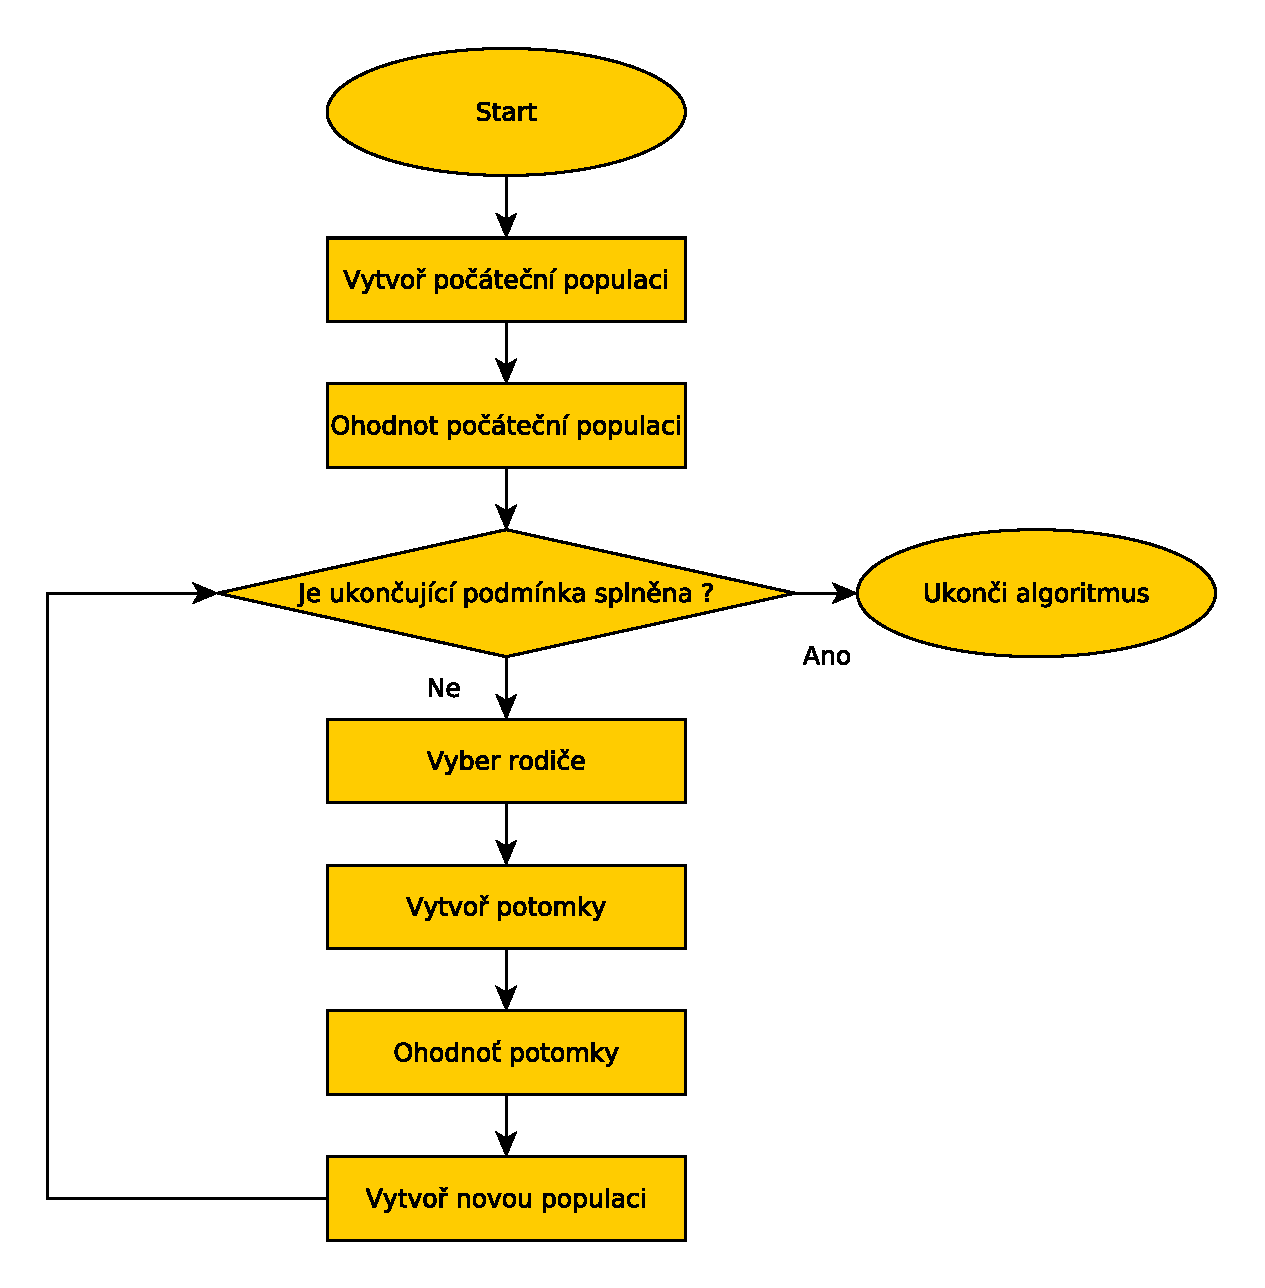
\includegraphics[scale=0.4]{fig/evolution_algorithm_flowchart}	
	\caption{Obecn� postup v�po�tu evolu�n�ho algoritmu}
	\label{fig:eaflow}
\end{figure}
%%%%%%%%%%%%% EVOLUTION ALGORITHM FLOWCHART %%%%%%%%%%%%%%%

\subsection{Fitness funkce}
Fitness funkce je obdoba ��elov� funkce z oboru matematick� optimalizace. N�zev fitness
poch�z� z oboru evolu�n� biologie, kde hodnota fitness popisuje biologickou zdatnost jedince
\cite{evolution_hardware}. Vstupem fitness funkce je (v jednodu���m p��pad�) jedinec
reprezentovan� chromozomem a v�stupem je hodnota reprezentuj�c� zdatnost jedince.

Ve slo�it�j��ch p��padech je nutn� rozli�ovat mezi prostorem genotyp� a fenotyp�. Genotypem
naz�v�me v kontextu evolu�n�ch algoritm� prostor v�ech mo�n�ch �e�en�, tedy 
v�ech mo�n�ch chromozom�. Fenotyp je soubor charakteristik, projev� a chov�n�,
jimi� se dan� jedinec reprezentovan� ur�it�m chromozomem projevuje.
Zobrazen� z prostoru genotyp� do prostoru fenotyp� lze potom vyj�d��t n�sledovn�:
$$ f_{phenotype} : U \to \mathcal{F}, $$
Potom je v�ak nutn� modifikovat na�i fitness funkci n�sledovn� :
$$ f : \mathcal{F} \to \mathcal{R} $$
a cel� proces evaluace jedince bude pot� kompizice t�chto dvou funkc� :
$$ f_{eval} = f \circ f_{phenotype}$$

Volba pota�mo n�vrh vhodn� fitness funkce je zna�n� obt��n�. Neexistuje ��dn� obecn�
p�edpis pro jejich n�vrh. Mus�me se spol�hat na obecn� pravidla, zku�enosti nebo 
intuici. Velk� mno�stv� dob�e zakomponovan�ch informac� o probl�m ve fitness funkci je
dobr�m z�kladem pro �sp�n� evolu�n� algoritmus. Obecn� tedy plat�, �e 
vhodn� zvolen� fitness funkce m� zna�n� dopad na kvalitu v�sledn�ho �e�en�.

\subsection{Zp�soby selekce}
Zp�soby selekce jsou d�le�it�m faktorem p�i n�vrhu evolu�n�ho algoritmu. Selekce
je proces, p�i n�m� se vyb�raj� rodi�e z aktu�ln� populace ur�en� k reprodukci. 
Dobr� selek�n� algoritmus mus� b�t schopen up�ednost�ovat jedince s vysokou hodnotou
fitness funkce, na druhou stranu mus� zajistit dostate�n� mno�stv� genetick�ho 
materi�l� pro dal�i generace. �asto vyu��van� selek�n� mechanismy, zejm�na v kontextu
genetick�ch algoritm� jsou nap��klad \cite{selection_schemes_comparison} :

\begin{itemize}
	\item \textit{deterministick� selekce}, kde se do mno�iny rodi�� vybere $k$
		jedinc� z aktu�ln� populace s nejvy��� hodnotou fitness,
		
	\item \textit{proporcionln� selekce}, kde pravd�podobnost v�b�ru jedince $i$ je 
		rovna vztahu $p_{i} = \frac{f(i)}{\sum_{j=1}{N} f(j)}$,
		
	\item \textit{turnajov� selekce}, kdy je v n�kolika kolech turnaje postupn� 
		porovn�no n�kolik n�hodn� vybran�ch jedinc� a v�t�z turnaje je za�azen
		do mno�iny rodi��. Turnaj provedeme $n$-kr�t, kde $n$ je po�adovan� mohutnost
		mno�iny rodi��. 
\end{itemize}

\subsection{Genetick� oper�tory}
Evolu�n� algoritmy vyu��vaj� k���en� i mutaci, oba mechanismy jsou p�evzaty z
oboru bun��n� biologie, kde se uplat�uj� v procesu reduk�n�ho d�len� bun�k.

Oper�tor mutace se aplikuje na potomka
a vytvo�� z n�j potomka mutovan�ho. Stejn� jako v biologii, mutace se vyskytuje
pouze v mal�m po�tu p��pad�. Na�im c�lem je prozkoumat prostor $U$ postupn� a
konvergovat k dobr�m �e�en�m. V p��pad� vysok� pravd�podobnosti mutace se ji�
nejedn� o algorigmus evolu�n�, n�br� revolu�n� a algoritmus p�ipom�n� 
sp��e n�hodn� prohled�v�n�.

Oper�tor mutace je velmi d�le�it�, nebo� zanesen�
n�hodne mutace zaji��uje nov� genetick� materi�l, ��m� je algoritmus jednou za
�as nucen prozkoumat vzd�len�j�� bod prostoru. Neuv�zne tak v lok�ln�ch extr�mech.

P�i k���en� doch�z� k p�enosu ��st� chromozom� rodi�� na potomka. Zp�sob� k���en�
existuje cel� �ada. Obecn� v�ak plat�, �e zp�sob k���en� je z�visl� na zvolen� 
reprezentaci. Pokud m�me jedince reprezentovan�ho grafem, oper�tor k���en� 
se bude zna�n� odli�ovat od p��padu, kdy m�me jedince reprezentovan�ho bin�rn�m
vektorem. 

Uve�m� si zde alespo� nejzn�m�j�� druhy k���en� nad bin�rn� reprezentaci, jimi� jsou:
\begin{itemize}
	\item \textit{jednobodov� k���en�}, kdy se ur�� m�sto k���en� ur�uj�c�,
		kter� ��st chromozomu doputuje do potomka.
		
	\item \textit{dvoubodov� k���en�} je obdobou v��e zm�n�n�ho, av�ak pro dva body
		k���en� a
	\item \textit{uniformn� k���en�}, kter� je do zna�n� m�ry zobecn�n�m v��e zm�n�n�ch.
		 Ur�� $n$ gen� v chromozomu, jejich� hodnoty jsou vyst��d�ny.
\end{itemize}

\subsection{N�vrh evolu�n�ho algoritmu}

Kvalita n�mi navr�en�ho evolu�n�ho algoritmu, je zejm�na z�visl� na n�sleduj�c�ch faktorech:
\begin{enumerate}
	\item reprezentace probl�m� a jeho k�dov�n�,
	\item pou�it� fitness funkce,
	\item zobrazen� z prostoru genotyp� do prostoru fenotyp�,
	\item volbou genetick�ch oper�tor� a zp�soby selekce,
	\item nastaven�m parametr� genetick�ho algoritmu.
\end{enumerate}

Prostor ka�d�ho probl�mu �e�iteln�ho evolu�n�my algoritmy je jin�. Neexistuje tedy obecn�
evolu�n� algoritmus, kter� by kvalitn� �e�il v�echny probl�my. Toto tvrzen� podporuje takzvan�
\textit{No Free Lunch} teor�m. Pokud uv��me dostate�n� velk� po�et optimaliza�n�ch probl�m�,
neexistuje ��dn� optimaliza�n� algoritmus, kter� projde ka�d� bod prostoru $U$ pr�v� jednou
a v pr�m�ru bude efektivn�j�� ne� ostatn� optimaliza�n� algoritmy \cite{nflteorem, evolution_hardware}. 
Z tohoto tvrzen� plyne, �e chceme-li �e�it optimaliza�n� probl�m skute�n� efektnivn�, mus�me 
do na�eho evolu�n�ho algoritmu vlo�it co nejv�ce informac� o �e�en�m probl�mu prost�ednictv�m 
zejm�na polo�ek zm�n�n�ch v��e.

\subsection{Genetick� algoritmy}

Evolu�n� algoritmy popisuj� mno�inu algoritm�, jejich� �innost je ur�ena procesem Darwinovsk�
evoluce. Na druh� stran� je v�ak neomezuje natolik, aby se od sebe nemohly (n�kdy i velmi
v�znamn�) li�it.

Asi nejv�znam�j��m ��stupcem evolu�n�ch algoritm� jsou genetick� algoritmy. Jediny jedn� populace
jsou reprezentov�ny �et�zcem (chromozomem) bin�rn�ch, celo��seln�ch nebo i re�ln�ch hodnot.
Inici�ln� populace vznik� bu� n�hodn� nebo za pou�it� vhodn� heuristiky. Jako selek�n� mechanismy
se zde uplat�uj� v�echny b�n�, stejn� tak zde najdeme pou�ity v�echny druhy metod k���en�.
Mutace se takt� pou��v�.

\subsection{Evolu�n� strategie}

Dal��m zaj�mav�m algoritmem jsou evolu�n� strategie. Jejich nejv�t�� zaj�mavost� je, �e
se spol�haj� pouze na oper�tor mutace. K���en� se zde nevyskytuje. Nov� generace se zde
vytv��ej� zejm�na tak, �e rodi�ovsk� je mutov�na p�i�ten�m hodnoty norm�ln�ho rozlo�en� s nulovou
$x' = x + \mathcal{N}(0, \sigma)$
st�edn� hodnotou. Rozptyl $\sigma$ se m�n� na z�klad� toho, jak dob�e algoritmus aktu�ln�
konverguje. Jako selek�n� mechanismy se u��v� tot�ln� elitismus ve variant�ch $(\mu + \lambda)$
a $(\mu. \lambda)$ \cite{ES}. Uva�ujeme-li $\mu$ mno�inu rodi�� a $\lambda$ mno�inu jejich
potomk�, pak :

\begin{itemize}
	\item $(\mu + \lambda)$ vybere do dal�� generace nejlep�� jedince z mno�iny
		rodi�� a potomku
	\item $(\mu, \lambda)$ vybere do dal�� generace jen ty nejlep�� potomky. Rodi�ovsk�
		generace tedy vym�r�.
\end{itemize} 

\section{Genetick� programov�n�}

Pro na�� pr�ce je zejm�na zaj�mav� genetick� programov�n�, nebo� pr�v� to jsme zvolili 
jako evolu�n� algoritmus pro �e�en� na�eho probl�m�. Sezn�m�me se s n�m podrobn�ji a 
proto mu v�nujme celou sekci.

Genetick� programov�n� je speci�ln�m druhem evolu�n�ho algoritmu, kde jednotlivce a 
cel� populace tvo�� po��ta�ov� programy. V�po�et iterativn� transformuje po��ta�ov�
programy na jin� po��ta�ov� programy aplikac� genetick�ch oper�tor�, kter� jsou 
pro genetick� programov�n� specializovan� specifick�. V�stupem genetick�ho algoritmu
je v p��pad�, �e usp�je, n�jak� program. 

\subsection{Reprezentace}
Evolvovan� programy mus�me vhodn� reprezentovat. Mus�me p�� tom kl�st d�raz na to,
�e programy je mezi sebou t�eba k���it, mutovat a obecn� na nich prov�d�t nutn�
genetick� operace. Na druh� stran� v�ak chceme volit takovou reprezentaci, kter�
n�m umo�n� programy evaluovat, tud�� vykon�vat je nad zadan�m vstupem. 

Jedinci v populaci jsou reprezentov�n� rad�ji jako \textit{abstraktn� syntaktick� stromy}
\cite{GPTutorial} ne� ��dky programu. Uk�zka jedince v genetic�m programov�n� je na
diagramu \ref{fig:exampletree1} a zobrazuje jedince reprezentovan�ho programem
\texttt{max(min(x,y), 5 + z)}. Stromy se skl�daj� z uzl� a list�. Listy jsou
reprezentov�ny termin�ln�m symbolem z mno�iny termin�l� $T$ a uzly jsou reprezentov�ny
funkc� z mno�iny $F$. Na diagramu \ref{fig:exampletree1} mno�inu funkc� tvo�� 
$F = \{max, min, +\}$ a mno�inu termin�lu $T = \{5, x, y, z\}$. Mno�iny povolen�ch
funkc� a termin�l� dohromady tvo�� primitivn� mno�inu syst�mu. Prostor mo�n�ch 
�e�en� m��eme tedy definovat jako mno�inu v�ech mo�n�ch strom�, kter� mohou vzniknout
kombinac� funkc� a termin�l� :

$$ U = \{t | t=(FT)^{n}, 0 \leq n \leq max\_depth \}$$

Programov� reprezentace strom� se li�� od programovac�ho jazyku. Plat� v�ak, �e 
v pros�ed�ch n�ro�n�ch na v�po�etn� v�kon je pam�ov� n�ro�nost grafov� reprezentace
neefektnivn�. Stromov� reprezentace lze u��t i nep��mo za pou�it� prefixov� notace.
P�� pou�it� prefixov� notace se z�vorky stanou nadbyte�n�mi a program lze v pam�ti
ulo�it jako \textit{line�rn� sekvenci symbol�}. Jako p��klad poslou�� diagram 
\ref{fig:exampletree1}, tedy \texttt{max min x y + 5 z}. Volba reprezentace tedy
v kone�n�m d�sledk� z�le�� na u�ivateli a jeho preferenc�ch, po�adavc�ch a prost�ed�. 

%%%%%%%%%%%%% TREE REPRESENTATION EXAMPLE 1 %%%%%%%%%%%%%%%
\begin{figure}[!ht]
	\centering
	\includegraphics[scale=0.6]{fig/example_tree1}	
	\caption{Uk�zka reprezentace programu max(min(x,y), 5 + z)}
	\label{fig:exampletree1}
\end{figure}
%%%%%%%%%%%%% TREE REPRESENTATION EXAMPLE 1 %%%%%%%%%%%%%%%

\subsection{Inicializace nult� populace}

Pro inicializaci nult� populace plat� obecn� pravidla. M��eme ji bu� volit n�hodn�
nebo pou��t n�jakou vhodnou heuristiku. Je zde v�ak specifick� vlastnost, kterou 
mus�me vz�t do �vahy. Na�e programy nemaj� pevn� omezenou velikost (d�lka
chromozomu je prom�nn�). Jak velk� n�hodn� programy tedy generovat ? Existuj� t�i
z�kladn� p��stupy:

\begin{enumerate}
	\item \textit{Full} metoda, kdy n�hodn� vygenerujeme strom do maxim�ln� povolen�
		hloubky,
	\item \textit{Grow} metoda, generujeme stromy prom�nliv� d�lky a tvaru (maxim�ln�
		hloubka je omezena) a
	\item \textit{Ramped half-and-half}, kdy polovina populace je generov�na metodou
		\textit{Grow} a druh� metodou \textit{Full}, za prom�nliv� maxim�ln� hloubky.
\end{enumerate}

Metoda Full v�dy a za v�ech okolnost� generuje pln� stromy. V uzlech jsou funkce
vyb�r�ny n�hodn� z mno��ny $F$ a jakmile algoritmus dos�hne maxim�ln� hloubky,
nageneruje termin�ly z mno�iny $T$ a skon��.

Grow metoda naproti tomu generuje v uzlech s ur�itou pravd�podobnost� i termin�ly, ��m�
je schopna vytv��et stromy r�zn�ch d�lek i tvar�. Je v�ak velmi z�visla na velikostech
mno�in $F$ a $T$. Pokud v�ak $|T| << |F|$ algoritmus degraduje na metodu Full. Pokud
na druh� stran� $|T| >> |F|$, algoritmus bude generovat jen velmi mal� stromy.

Aby se omezil dopad rozd�ln�ch velikost� mno�in $T$ a $F$, John Koza navrhl alternativu
v podob� algoritmu ramped half-and-half. Ten pou��v� ob� metody sou�asn� na polovinu 
jedinc� populace a maxim�ln� hloubku stromu vol� n�hodn�, ��m� zaji��uje prom�nlivou
velikost i tvar strom�.

\subsection{Genetick� oper�tory a selekce}

V p��pad� selekce do mno�iny rodi��, se vyu��vaj� v�echny b�n� selek�n� mechanismy
zn�me z evolu�n�ch algoritm�, av�ak nej�ast�ji se vyu��v� turnajov� selekce n�sledovan�
proprcion�ln� selekc�.

Zaj�mav�j�� je to v p��pad� genetick�ch oper�tor� k���en� a mutace. Nej�ast�j�� formou
k���en� je \textit{podstromov� k���en�}. U rodi�� vybran�ch k reprodukci se se n�hodn� 
vybere bod k���en�, kter� v genetick�m programov�n� zastupuj� v�tve stromu. Potomek
vznikne um�st�n�m podstromu prvn�ho rodi�e na pr�zdnou v�tev druh�ho rodi�e (rodi�e
implicitn� zachov�v�me). Cel� proces bl��e ilustruje diagram \ref{fig:tree_crossover}

%%%%%%%%%%%%% TREE CROSSOVER EXAMPLE 1 %%%%%%%%%%%%%%%
\begin{figure}[!ht]
	\centering
	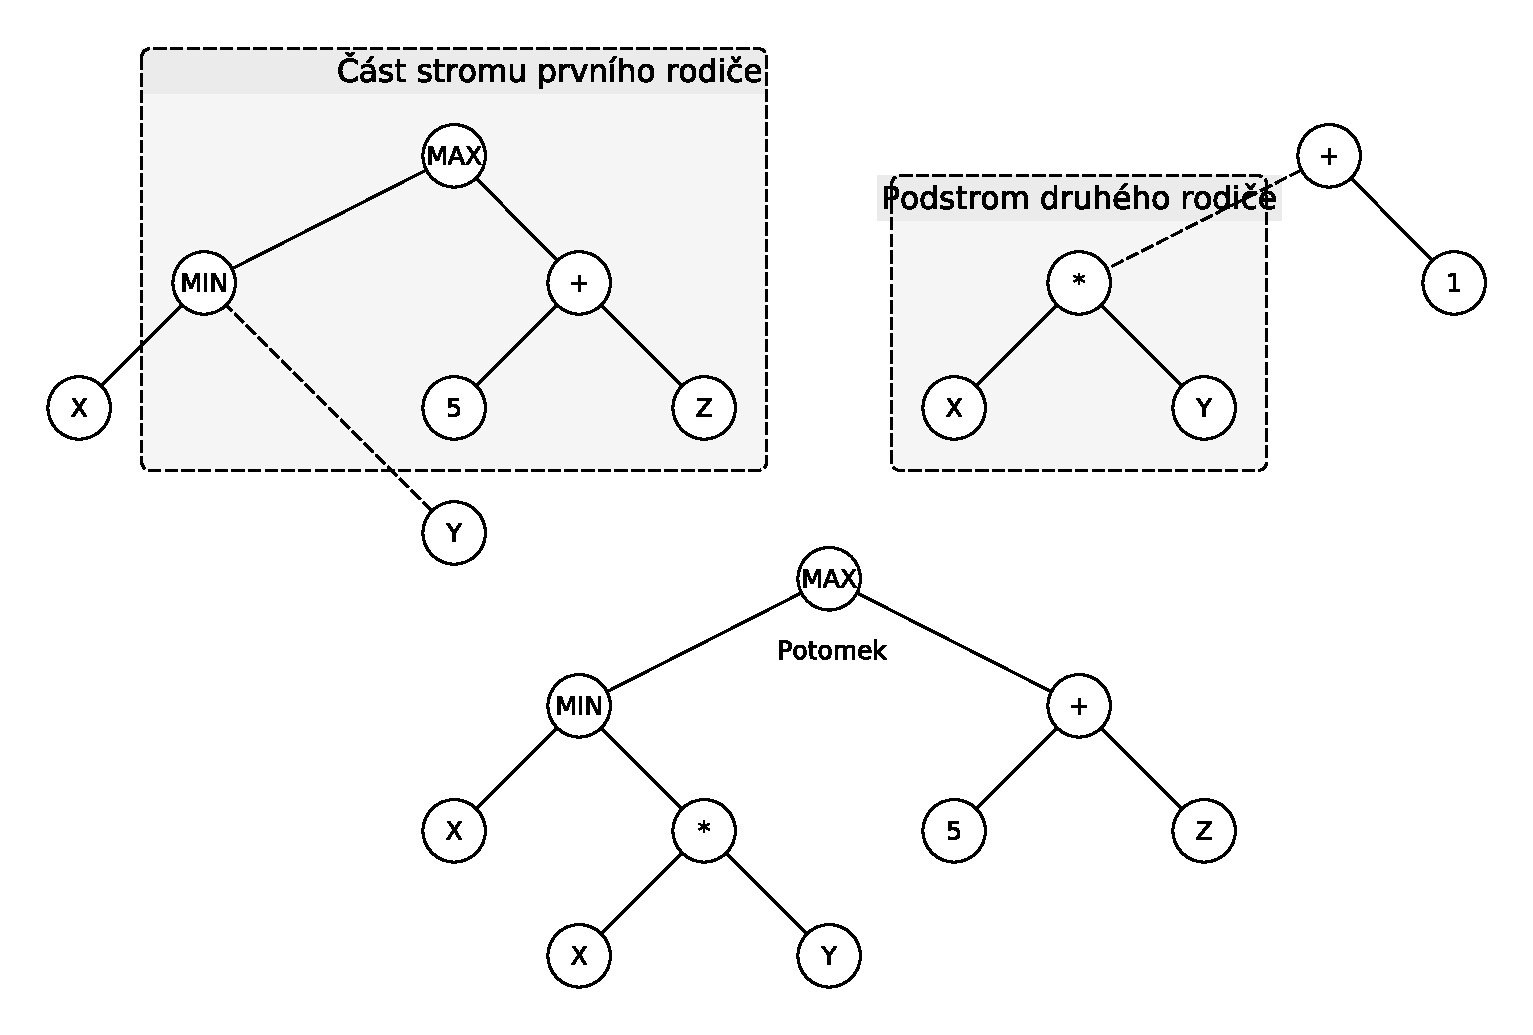
\includegraphics[scale=0.6]{fig/tree_crossover}	
	\caption{Uk�zka oper�toru podstromov�ho k���en�}
	\label{fig:tree_crossover}
\end{figure}
%%%%%%%%%%%%% TREE CROSSOVER EXAMPLE 1 %%%%%%%%%%%%%%%

Je vid�t, �e k���en� vytvo�� pouze jednoho potomka. Pro v�ce potomk� cel� proces 
opakujeme. Dale existuje specializace podstromov�ho k���en�, obdoba jednobodov�ho
k��en�, kdy se ur�� v obou rodi��ch stejn� bod k���en� a p�ehozen� koresponduj�c�ch
podstrom�. Je v�ak pot�eba oba strommy proj�t a naj�t spole�n� region, tedy ��st stromu,
kde je mo�n� k���it. Existuj� dal�� varianty jako je k���en� se zachov�n�m kontextu, 
velikost zachov�vaj�c� k���en� a uniformn� k���en�. T�mito se zde zat�m bl��e zab�vat
nebudeme.

Nejb�n�j�� druh mutace je podstromov� mutace. Algoritmus podstromov� mutace ve stromu
n�hodn� zvol� v�tev z n�� n�hodn� vygeneruje nov� podstrom, jak ilustruje diagram
\ref{fig:subtree_mutation}. V p��pad� tohoto algoritmu jde v podstat� o alternativu k
podstromov�mu k���en� s jedn�m rodi�em a jedn�m n�hodn� generovan�m stromem.

Dal�� variantou mutace v genick�m programov�n� je uzlov� nutace, kdy na ka�d�
uzel stromu je s ur�itou nizkou pravd�podobnost� mutace aplikov�na. Star� uzly
se nahrazuj� nov�mi se stejnou aritou.

%%%%%%%%%%%%% SUBTREE MUTATION EXAMPLE 1 %%%%%%%%%%%%%%%
\begin{figure}[!ht]
	\centering
	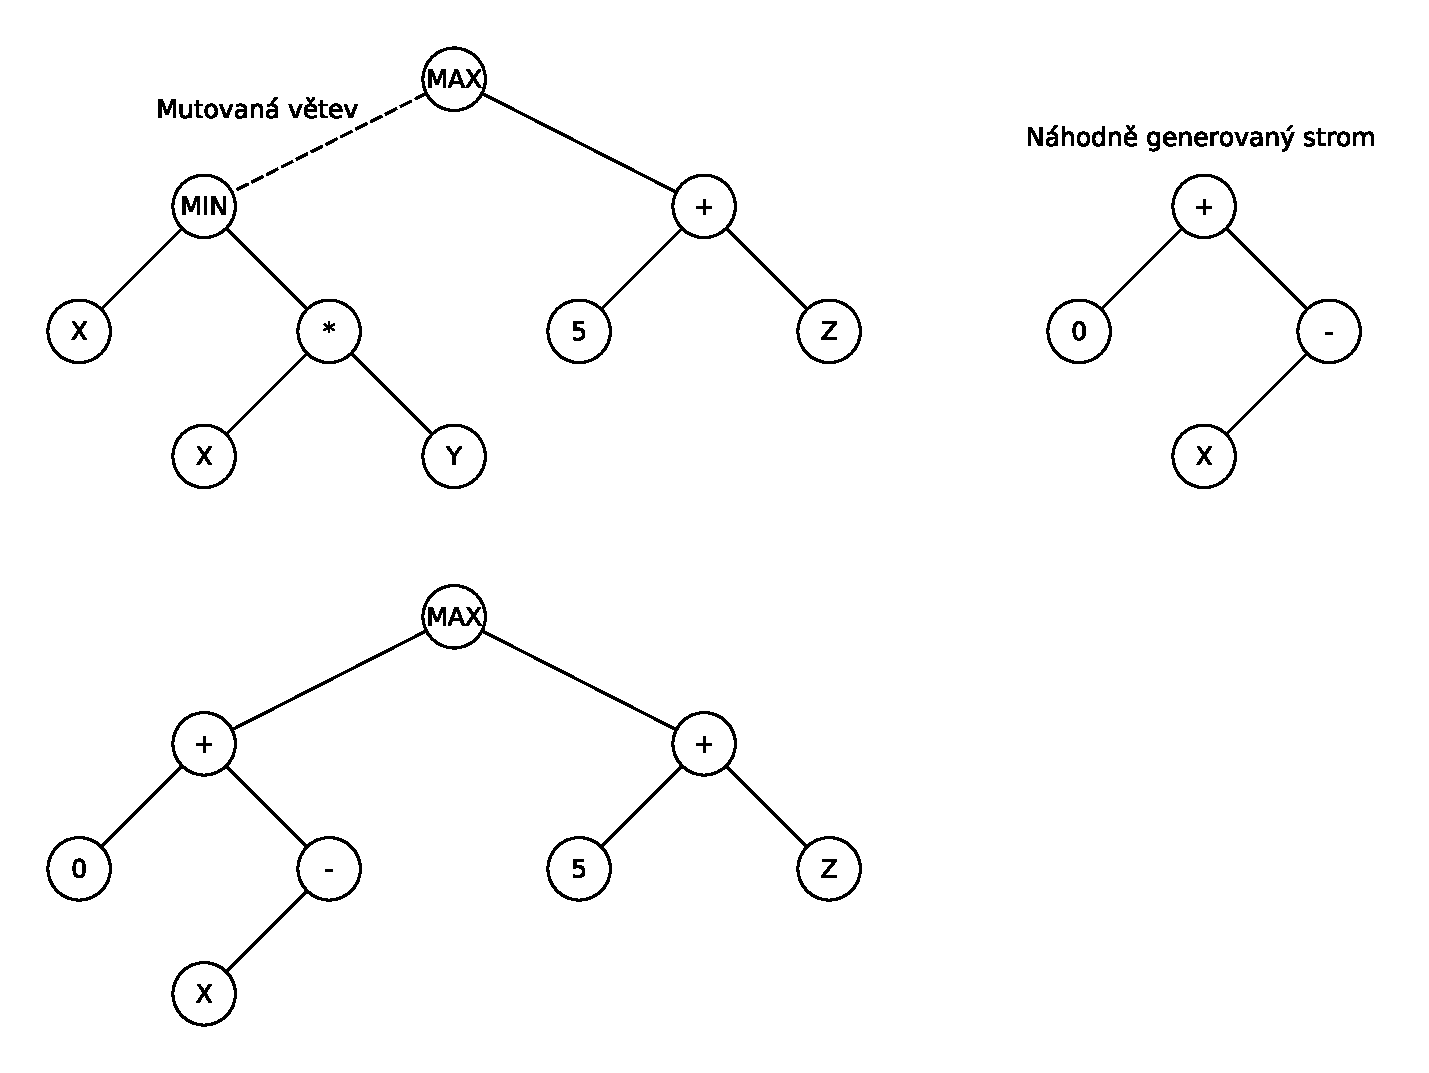
\includegraphics[scale=0.6]{fig/subtree_mutation}	
	\caption{Uk�zka oper�toru podstromov� mutace}
	\label{fig:subtree_mutation}
\end{figure}
%%%%%%%%%%%%% SUBTREE MUTATION EXAMPLE 1 %%%%%%%%%%%%%%%

\subsection{Fitness funkce}
Populace v genetick�m programov�n� jsou programy. Evaluace kvality programu se prov�d�
zpravidla spu�t�n�m dan�ho programu nad dan�m vstupem a ohodnocen�m v�stupu. Spu�t�n� 
programu nad zadan�m vstupem m��eme ch�pat jako zobrazen� z mno��ny genotyp� do mno�iny
fenotyp� za vstupu dal��ho parametru. Cel� proces evaluace m��e b�t tedy ch�p�n jako :
$$ f_{eval} = f \circ f_{run}(input)$$
kde $f$ je standarn� fitness funkce a $f_{run} : (I \times U) \to \mathcal{F}$ je
modifikovan� zobrazen� genotyp-fenotyp pro n�jak� vstup $I$.

Fitness funkce v p��pad� genetick�ho programov�n� se li�� od t� tradi�n� v jednom
d�le�it�m sm�ru. Proto�e pracujeme nad programy, mus�me poskytnout zp�sob, jak dan�
program spustit. Mo�nost� by bylo program zkompilovat. To s sebou nese zna�nou re�ii
a tak toto �e�en� nen� v mnoha p��padech vhodn�. Pokud v�ak bychom dan� program cht�li
evaluovat n�kolikr�t (mnohokr�t), M��e se i toto �e�en� jevit jako vhodn�.

�ast�j�� je ale programy interpretovat, to znamen� proj�t strom od list� ke ko�enu a 
spo��t�n� hodnoty uzlu za vstupu hodnot jeho n�sledn�k�. Kostru algoritmu bude jist�
tvo�it pr�chod postorder. Evaluace jednotliv�ch hodnot v�ak nemus� b�t za v�ech 
okolnost� trivi�ln�, m��e nap��klad nastat p��pad, kdy bude program d�lit nulou nebo
se sna�it se��st hodnoty r�zn�ch typ� (nap�. \texttt{Bool} a \texttt{Int}). Proto
se po prvc�ch mno�iny $F$ vy�aduj� dv� uz�v�rov� vlastnosti. 

\begin{enumerate}
	\item \textit{typov� konzistence} a
	\item \textit{bezpe�nost p�� evaluaci}.
\end{enumerate}

Typov� bezpe�nost je nutn� zejm�na kv�li oper�toru k���en�, proto�e ten nebere typy 
v potaz. Mus�me tedy po��tat s t�m, �e jak�koli podstrom m��e b�t zav�en jako argument
libovoln� funkce z mno�ny $F$ a v�sledn� program p�esto mus� b�t interpretovateln�.
Jin�mi slovy navratov� typ libovoln� funkce z mno�iny $F$ mus� b�t stejn� jako
typ libovoln�ho vstupn�ho argumentu jak�koli dostupn� funkce. Toho m��eme dos�hnout
nap��klad jednodu�e t�m, �e v�echny funkce z mno�iny $F$ budou definov�ny na jedn�m
oborem hodnot toto�n�ho typu. �asto to v�ak nen� mo�n�, proto se mus�me n�kdy uch�lit
nap��klad k implicitn�m typov�m konverz�m, nebo k otypov�n� funkc� a typov� bezpe�n�
operaci k���en�.

Dal�� vlastnost�, kterou je nutn� splnit je, abychom se vypo��dali s mo�n�mi
nedefinovan�mi hodnotami, kter� jsou typick� pro vstupy n�kter�ch parci�ln�ch funkc�
jako je d�len�, kde hodnota je nedefinovan� pokud je d�litel roven nule.
S parci�ln�mi funkcemi se m��eme vypo��dat t�m, �e je explicitn� roz����me na funkce
tot�ln� nebo v p��pad�, je-li nedefinovan� hodnota detekov�na, zna�n� sn���me jedinc�v 
fitness.


\chapter{N�vrh �e�en�}
\label{sec:solution_design}

\chapter{Z�v�r}
%=========================================================================
% Conclusion for Marek Kidon's thesis



%=========================================================================


%=========================================================================
 % viz. obsah.tex

  % Pouzita literatura
  % ----------------------------------------------
\ifslovak
  \makeatletter
  \def\@openbib@code{\addcontentsline{toc}{chapter}{Literatúra}}
  \makeatother
  \bibliographystyle{czechiso}
\else
  \ifczech
    \makeatletter
    \def\@openbib@code{\addcontentsline{toc}{chapter}{Literatura}}
    \makeatother
    \bibliographystyle{czechiso}
  \else 
    \makeatletter
    \def\@openbib@code{\addcontentsline{toc}{chapter}{Bibliography}}
    \makeatother
    \bibliographystyle{plain}
  %  \bibliographystyle{alpha}
  \fi
\fi
  \begin{flushleft}
  \bibliography{literatura} % viz. literatura.bib
  \end{flushleft}

  % Prilohy
  % ---------------------------------------------
  \appendix
\ifczech
  \renewcommand{\appendixpagename}{Přílohy}
  \renewcommand{\appendixtocname}{Přílohy}
  \renewcommand{\appendixname}{Příloha}
\fi
\ifslovak
  \renewcommand{\appendixpagename}{Prílohy}
  \renewcommand{\appendixtocname}{Prílohy}
  \renewcommand{\appendixname}{Príloha}
\fi
  \appendixpage

\ifslovak
  \section*{Zoznam príloh}
  \addcontentsline{toc}{section}{Zoznam príloh}
\else
  \ifczech
    \section*{Seznam příloh}
    \addcontentsline{toc}{section}{Seznam příloh}
  \else
    \section*{List of Appendices}
    \addcontentsline{toc}{section}{List of Appendices}
  \fi
\fi
  \startcontents[chapters]
  \printcontents[chapters]{l}{0}{\setcounter{tocdepth}{2}}
  \chapter{Obsah CD a manuál pro spuštění a vyhodnocení experimentů}

Přiložené CD obsahuje zdrojové texty k této práci, 


\chapter{Článek a plakát na konferenci Excel@FIT 2016}
Předběžné výsledky této práce byly publikovány na konference Excel@FIT 2016. Příspěvek byl vybrán
odbornou komisí k ústní prezentaci. Práce získala ocenění odborného panelu za nekonvenční přístup k návrhu hašovacích
funkcí pomocí evolučního algoritmu a ocenění odbornou veřejností za excelentní práci a její prezentaci během přehlídky.

\newpage
\begin{figure}[!ht]
	\centering 
	\includepdf[pages=1]{includes/ExcelFITPaper.pdf}
\end{figure}
\newpage
\begin{figure}[!ht]
	\centering 
	\includepdf[pages=2]{includes/ExcelFITPaper.pdf}
\end{figure}
\newpage
\begin{figure}[!ht]
	\centering 
	\includepdf[pages=3]{includes/ExcelFITPaper.pdf}
\end{figure}
\newpage
\begin{figure}[!ht]
	\centering 
	\includepdf[pages=4]{includes/ExcelFITPaper.pdf}
\end{figure}
\newpage
\begin{figure}[!ht]
	\centering 
	\includepdf[pages=5]{includes/ExcelFITPaper.pdf}
\end{figure}
\newpage
\begin{figure}[!ht]
	\centering 
	\includepdf{includes/ExcelFITPoster.pdf}
\end{figure}

 % viz. prilohy.tex
\end{document}
